\documentclass[12pt,a4paper,leqno]{article}

\usepackage[utf8]{inputenc}
\usepackage[T1]{fontenc}
\usepackage[english]{babel}
\usepackage{amsthm}
\usepackage{amsfonts}         
\usepackage{amsmath}
\usepackage{amssymb}
\usepackage{hyperref}
\usepackage[all]{hypcap}
\usepackage{tikz}
\usetikzlibrary{matrix, arrows, decorations.pathmorphing}

\newcommand{\R}{\mathbb{R}}
\newcommand{\C}{\mathbb{C}}
\newcommand{\Q}{\mathbb{Q}}
\newcommand{\N}{\mathbb{N}}
\newcommand{\No}{\mathbb{N}_0}
\newcommand{\Z}{\mathbb{Z}}
\newcommand{\OO}{\mathcal{O}}
\newcommand{\diam}{\operatorname{diam}}

\newcommand{\cat}{\mathcal}
\newcommand{\isomto}{\stackrel{\sim}{\rightarrow}}
\newcommand{\coker}{\mathrm{coker}}
\newcommand{\im}{\mathrm{im}}
\newcommand{\coim}{\mathrm{coim}}
\newcommand{\spec}{\mathrm{Spec}}
\newcommand{\plim}{\varprojlim}
\newcommand{\dlim}{\varinjlim}


\newcommand{\sectionbreak}{\clearpage}

\newcommand{\fref}[1]{\hyperref[{#1}]{\ref*{#1}}}


\newtheorem{theo}{Theorem}[section]
\theoremstyle{plain}
\newtheorem{thm}[theo]{Theorem}
\newtheorem{lem}[theo]{Lemma}
\newtheorem{prop}[theo]{Proposition}
\newtheorem{cor}[theo]{Corollary}

\theoremstyle{definition}
\newtheorem{defn}[theo]{Definition}
\newtheorem{con}[theo]{Conjecture}
\newtheorem{ex}[theo]{Example}

\theoremstyle{remark}
\newtheorem{rem}[theo]{Remark}

\pagestyle{plain}
\setcounter{page}{1}
\addtolength{\hoffset}{-1.15cm}
\addtolength{\textwidth}{2.3cm}
\addtolength{\voffset}{0.45cm}
\addtolength{\textheight}{-0.9cm}

\title{Resolution of Singularities}
\author{Toni Annala}
\date{}

\begin{document}

\maketitle

\tableofcontents

\section{Introduction}

For many of the most important theorems in mathematics giving even an approximate idea of what the theorem states is fairly hard. This is not the case with resolution of singularities. The basic idea is very geometric, and can be easily stated approximately assuming very little prior mathematics background. It is a statement considering varieties, i.e., solution sets of equation systems consisting entirely of polynomial equations.

Let us start with an example. The solution set for the equation $y^2 - x^3$ is visualized in Figure \fref{cusp1}. At every point of the curve, except at the origin, the curve seems to be smooth, i.e., if we zoom close enough, it starts looking like a straight line. These kind of points are called \emph{nonsingular} or \emph{regular points}. More generally in higher dimensional varieties (say the dimension is $n$) we would consider a point to be nonsingular if locally around it the variety looks like the ''normal'' $n$-dimensional space (you can think of $\R^n$ if we are dealing with real solutions, $\C^n$ if with complex solutions).  

But something weird happens at the origin: the direction of the curve ''changes'' suddenly, and no matter how close we try to zoom, the curve will never start looking like a straight line. Points that fail to be nonsingular are called \emph{singularities} or \emph{singular points}. The type of curve singularity we have in Figure \fref{cusp1} is called a \emph{cusp}.

\begin{figure}\label{cusp1}
\begin{center}
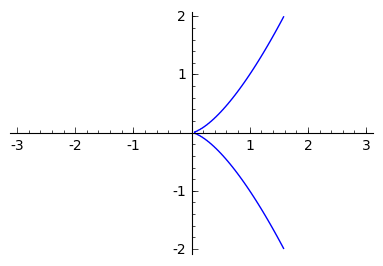
\includegraphics{pics/cusp.png}
\caption{A cusp.}
\end{center}
\end{figure}

Now a question arises: would it be possible to parametrize our singular curve $C$ with another, nicer, curve: could we parametrize the points of $C$ with points of a nonsingular curve $C'$ (meaning that it has no singular points)? In the above case it is indeed possible. Take the curve $C'$ that is the zero set of the polynomial equation $y'^2 - x'$ plotted in Figure \fref{nsing1}. We would like to define a map $C' \to C$. Send a point $(x',y') \in C'$ to $(x',y'x')$. This point lies in $C$ as
\begin{align*}
\left( y'x' \right) ^ 2 - x'^3 = x'^2 (y'^2 - x'),
\end{align*}
and the right hand side is zero by assumption. Hence we have what we desired: a parametrization of the curve $C$ by a nonsingular curve $C'$.

\begin{figure}\label{nsing1}
\begin{center}
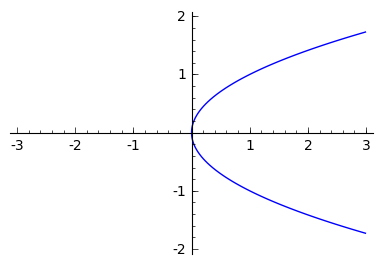
\includegraphics{pics/parabola.png}
\caption{The solution set for $y'^2 - x' = 0$.}
\end{center}
\end{figure}

Before going further, let us have another example. The equation $y^2 - x^3 - x^2$ gives the curve visualized in Figure \fref{node1}. The origin is clearly singular, but this singularity is different from the one we had in Figure \fref{cusp1}. The curve intersects itself! Luckily this self-intersection is in some sense as good as possible, at least the different branches meet \emph{transversally}, i.e., they have distinct tangent lines. A singular point, where two branches of a curve meet transversally is called a \emph{node}. 

Can we find a nonsingular parametrization for this curve? Yes we can. Take the curve $y'^2 - x' - 1$, which is visualized in Figure \fref{nsing2}. A parametrization is again given by $(x', y') \mapsto (x', x'y')$ which can be checked with similar reasoning as before.

\begin{figure}\label{node1}
\begin{center}
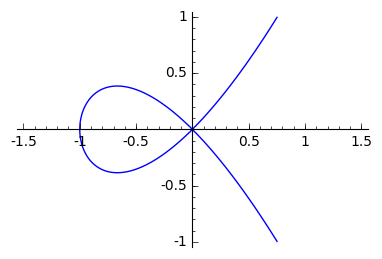
\includegraphics{pics/node.png}
\caption{This kind of singularity is called a \emph{node}.}
\end{center}
\end{figure}

\begin{figure}\label{nsing2}
\begin{center}
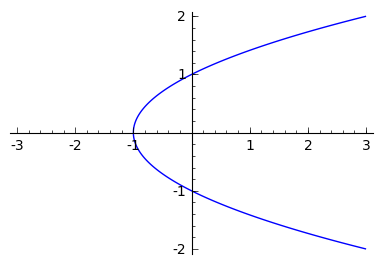
\includegraphics{pics/parabola2.png}
\caption{I swear, a parabola is not going to \emph{always} work.}
\end{center}
\end{figure}

Finding a parametrization of a singular variety by a nonsingular one is called \emph{resolving} its singularities (this is not what one usually means by it, usually we would require the parametrizing curve to be isomorphic to the original one almost everywhere). The problem of resolution of singularities simply asks whether or not the singularities of any variety can be resolved. It is also of some interest if there is a systematic way of doing this.

\subsection{A condenced historical account of the problem}

Although the problem is much older, we start with Oscar Zariski. Zariski was arguably the leading algebraic geometer of the first half of the twentieth century: if Grothendieck is to be regarded as the father of modern algebraic geometry, then Zariski is the grandfather. He did his undergraduate studies in Kiev, and later moved to do his doctorate in Rome under Guido Castelnuovo. During his graduate studies he was very much influenced by what is now known as the Italian school of classical algebraic geometry, which is nowdays notorious for their usage of ''geometric intuition'' leading to some false proofs and untrue theorems.

But Zariski was more algebraically inclined than his Italian teachers. And even though he enjoyed the geometric way of thinking of the Italians, he also had some worries concerning their rigour. Because of these, Castelnuovo once stated: ''Zariski, you are here with us but are not one of us'' \cite{Par}. This was not meant in a bad way, the methods of the Italian school had reached a dead-end, and would no longer be able to accomplish significant progress in the field, and Castelnuovo knew this all too well. But it would still take years before Zariski would start systematically rebuilding the foundations of algebraic geometry.

In 1932, now in the United States, Zariski began to work on his monograph \emph{Algebraic Surfaces}, a task that would take him three years. The purpose of the monograph was to give a complete account of the results concerning algebraic curves obtained by the Italian school with rigorous proofs. However, while writing the book, he became increasingly certain that the entire foundations of algebraic geometry should be completely rebuilt using commutative algebra. He later stated himself: ''working on that book took all my time because as I worked I became more and more disgusted with the kind of proofs that the Italian geometers were giving, and I started studying algebra seriously.'' \cite{Par} He started incorporating recent results from commutative algebra achieved mainly by Noether, Krull and Dedekind, and casting everything in algebraic geometry in terms of the theory of commutative rings and their ideals. 

After the completion of the monograph in 1935, Zariski went on to develop an abstract theory of algebraic geometry over an arbitrary (algebraically closed) ground field (instead of the coordinates of the points being complex numbers, they could be elements of some abstract field). It was during this time when he got interested in the resolution problem. The problem of resolution of singularities for higher dimensional varieties had long stood open, and many good mathematicians had given it a shot. Only some partial results had been achieved, and these were over complex numbers.

Zariski gave a simple proof for the resolution problem for surfaces using his notion of \emph{normalization}, a term that should ring a bell to anyone who has studied algebraic geometry or commutative algebra. Resolution for surfaces is more complicated than for curves as the singularities of a surface need not to be confined in a finite set of points: the singular points can form curves as well. Normalizing a variety produces a variety whose singularities are of codimension two, which, in the case of surfaces, means that all singularities are point-singularities, i.e., the earlier complication is now gone! After normalization, resolving the singularities was fairly straightforward.

The resolution of singularities for surfaces had, however, essentially already been solved by the Italian algebraic geometers \cite{Par}. But Zariski didn't stop there. Later, he was able to show that the singularities of three-folds (three dimensional varieties) over a field of characteristic zero (three dimensional varieties) can be resolved. This was a problem that had completely eluded the approaches of the Italian school, and was also the moment that proved to rest of the world how powerful algebraic methods could be in algebraic geometry.

This is however where the contributions of Zariski (essentially) end. For further progress some time had to pass, and another rebuilding of the foundations of algebraic geometry had to happen. Alexander Grothendieck, motivated by the famous Weil conjectures linking together number theory and geometry, began a systematic rebuilding of the whole field in mid 50s. The result was a very powerful theory of algebraic geometry, whose level of abstraction was something previously unseen in mathematics. Even Mumford, a student of Zariski who won the Fields medal in 1974, stated the following in a letter to Grothendieck: ''... I should say that I find the style of the finished works, esp. EGA, to be difficult and sometimes unreadable, because of its attempt to reach superhuman level of completeness.'' \cite{Mum} One can only imagine the struggle for those mathematicians that weren't quite as good as Mumford when trying to learn the theory. Such was the power of this theory, however, that the theory became universally accepted rather quickly.

At the time, resolution of singularities was considered one of the most important open problems in algebraic geometry, for it would enable one to transfer many questions concerning singular varieties to questions involving only nonsingular ones, which are better understood. Even Grothendieck considered the problem to be one of the two most important ones, alongside his standard conjectures (which, to this day, remain open).

In the 60s Heisuke Hironaka, another student of Zariski to be given the Fields medal, decided to attack the resolution problem. Zariski himself never truly tried to deploy the Grothendieck style of algebraic geometry. This was probably because of the great time investment required in order to learn to use it, combined with the fact that his own research was going well enough. \cite{Par} But Hironaka, like many of the students of Zariski, fully endorsed this new theory. With the new tools given by the theory of schemes, he was able to do what Zariski himself had tried and failed: in the famous paper published in 1964 in Annals of Mathematics, Hironaka gave a complete proof for resolution of singularities over a ground field of characteristic zero. 

The proof, originally around 200 pages long, quickly gained a reputation for being extremely complicated and hard to understand. However, in further research the proof has been simplified and shortened considerably. For example in \cite{Wlo} W\l{}odarczyk gives a self contained proof for resolution of singularities via a Hironaka-style argument in around twenty pages! An overview of a Hironaka-style argument for proof of resolution of singularities in characteristic 0 is given in Section \fref{HirRes}.

This still left open the finite characteristic case important in many applications to number theory. Partial results were obtained by Shreeram Abhyankar, another student of Zariski, who in 1966 published a proof for resolution of singularities for three-folds over algebraically closed fields of finite characteristic different from $2,3$ and $5$ \cite{HLOQ}. He later on went to generalize his result for three-folds in characteristic $2,3$ and $5$, as well as giving a proof for resolution of singularities for arithmetic surfaces.

However, for a long time essentially no progress was made. Hironaka's argument resisted all attempts of generalization to finite characteristic, and all algebraic approaches in the spirit of Zariski and his students seemed to fail as well. The initial success of the algebraic approach had blinded almost the entire field into thinking that this was the right way. The spell was finally broken by a young Dutch mathematician Aise Johan de Jong, who in a 1995 talk gave an outline for a very geometric proof for resolving singularities by means of so called alterations. 

His proof, published in a 1996 article \cite{Jong}, worked just as well over finite characteristic. A circle had closed: first algebra had had to replace geometry when geometrical methods failed, and now geometry, when all algebraic approaches seemed to fail, replaced algebra. Perhaps the most striking trait of his proof was the fact that essentially everything needed was already well known for nearly twenty years before the proof \cite{HLOQ}, the ingenious part was how the results were put together.

The resolution given by alterations is not, however, a resolution in the traditional sense. Traditionally one wants the resolution to produce a variety that is \emph{birational} to the original variety, i.e., it is isomorphic to the original variety outside some small subset. What de Jongs method gives is more like some kind of finite cover. But for many of the applications this is enough. The traditional problem of resolution of singularities in finite characteristic remains open.


\section{Completions}

In this section we will talk about completing a commutative local ring. Completion, together with localization, form a very powerful way of looking at the structure of an algebraic variety near a point. Familiarity with basic algebraic geometry and commutative algebra is assumed.

We begin with a motivating example. Recall the nodal curve $C$ from the first section, defined as the solution set of the polynomial $y^2 - x^3 - x^2$. At the origin the curve intersects itself, and it seems like the curve should, at least near the origin, consist of two components. But as $y^2 - x^3 - x^2$ is an irreducible polynomial, the coordinate ring $\OO_C (C)$ is an integral domain, as is the localization $\OO_{C,p}$ at origin $p$.

\begin{figure}\label{node2}
\begin{center}
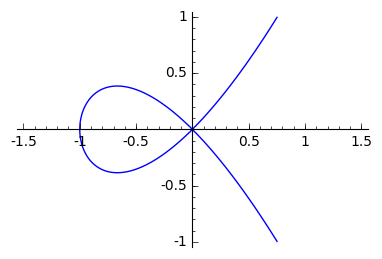
\includegraphics{pics/node.png}
\caption{The nodal curve.}
\end{center}
\end{figure}

This can be thought in the following way. The open sets of the Zariski topology are just the curve $C$ minus finitely many points, so they contain almost all of the curve $C$. The localization at origin gives essentially all information about the curve $C$ found in arbitrarily small neighbourhoods of the origin, and as none of these is small enough to make $C$ irreducible, the localization stays irreducible. It is as if algebra doesn't allow us to see close enough.

Of course analytically we may break the curve into to branches: the equation of the curve
\begin{equation*}
y^2 = x^3 + x^2
\end{equation*}
can be solved to give
\begin{equation*}
y = \pm \sqrt{x^3 + x^2} =  \pm x \sqrt{1+x},
\end{equation*}
describing the two branches of the curve.

We may connect this back to algebraic geometry when we note that $\sqrt{1+x}$ can be expressed by its Taylor series. Hence, if we think $y^2 - x^3 - x^2$ as an element of the formal power series ring $k[[x,y]]$ instead of the polynomial ring $k[x,y]$, the equation $y^2 - x^3 - x^2$ cuts out a reducible subscheme of $\spec k[[x,y]]$, and the irreducible components correspond to the two branches at the origin. Somehow, when we passed into the ring of formal power series, we are now much closer to the origin than by localization. 

As $k[[x,y]]$ is a local ring with maximal ideal $(x,y)$, the localization $k[x,y]_{(x,y)}$ embeds into it, and from this it is fairly easy to see that $\OO_{C,p}$ embeds into $k[[x,y]]/(y^2 - x^3 - x^2)$. The idea of completion of local rings is exactly this: we want to get closer, so instead of just looking at the localization, we somehow replace the local ring with some sort of power series ring. We say that we pass into \emph{formal neighbourhood} of a point $p$ when we do this. The nice thing is that these are usually much simpler than the local rings: for example, if we have a nonsingular $k$-variety $X$ of dimension $d$, where $k$ is algebraically closed, then the completion $\widehat \OO_{X,p}$ of the local ring at a closed point $p$ is isomorphic to $k[[x_1,...,x_d]]$.

\subsection{Completion of topological abelian groups}

Let $G$ be a topological abelian group. We say that a sequence $(x_i)$ in $G$ is \emph{Cauchy sequence} if for all neighbourhoods $U$ of $0$ we have $N_U \in \N$ such that $x_i - x_j \in U$ for all $i,j \geq N_U$. We say that $G$ is \emph{complete} if all Cauchy sequences converge to some value in $G$.

\begin{defn}
Let $G$ be a topological abelian group. The \emph{completion} of $G$, denoted by $\widehat G$, is ''the smallest complete group where $G$ can be mapped into''. More precisely, this means that completion is a continuous group morphism $G \to \widehat G$, where $\widehat G$ is complete, and for all continuous homomorphisms $G \to X$, where $X$ is complete, we have a unique morphism such that the following diagram commutes:

\begin{center}
\begin{tikzpicture}[scale=1]
\node (G) at (0,0) {$G$};
\node (Ghat) at (0,2) {$\widehat G$};
\node (X) at (3,2) {$X$};


\path[]
(G) edge[->] (Ghat)
(G) edge[->] (X)
(Ghat) edge[->, dashed] node[above]{$\exists !$} (X)
;
\end{tikzpicture}
\end{center}
It is clear that this defines $\widehat G$ up to unique isomorphism, if it exists.
\end{defn}

Next we will show that the completion always exists when $G$ is first countable and Hausdorff. The idea is exactly the same one that is used when completing metric spaces.

Denote by $s(G)$ the set of Cauchy sequences in group $G$. This is a group: if $(x_i)$ is a Cauchy sequence, then so is $(-x_i)$ for negation is homeomorphism. If $(x_i)$ and $(y_i)$ are Cauchy sequences, then so is $(x_i + y_i)$. This is not too hard to see: for all neighbourhoods $U$ of the origin, we have smaller neighbourhoods $V_1$ and $V_2$ such that $V_1 + V_2 \subset U$ by continuity of summation. Then we may choose $N$ to be large enough so that $x_i-x_j \in V_1$ and $y_i-y_j \in V_2$ for all $i,j \geq N$. Now $(x_i + y_i) - (x_j + y_j) = (x_i - x_j) + (y_i - y_j) \in U$. Similarly we can see that $s_0(G)$, the sequences of $G$ that converge to 0, is a subgroup of $s(G)$. We define a topological group $G'$ algebraically as $s(G) / s_0(G)$.

Next we define $G'$ topologically. For every neighbourhood $U$ of 0, let $U' \subset G'$ consist of those equivalence classes $[(x_i)]$ for which there exists a neighbourhood $\epsilon$ of origin, such that $x_i + \epsilon \subset U$ for $i \gg 0$. This is clearly independent of the choice of the representative $(x_i)$. This forms a neighbourhood basis for $0$ in $G'$ inducing a structure of a topological group, as the next lemma shows. 

\begin{lem}\label{TopGroupFromNbhd}
The open sets $U'$ define a structure of a topological group on $G'$ when we give $G'$ the topology where the open sets are of form
\begin{equation*}
\{O \subset G \mid \mathrm{for \ all \ } x \in G \mathrm{\ we \ have \ } U' \mathrm{\ s.t. \ } x+U' \subset O \}.
\end{equation*}
In this topology $U'$ form a neighbourhood basis for $0$ (we do not yet claim these to be open, although it is true).
\end{lem}
\begin{proof}
From basic properties of topological groups, it suffices to show that the following three properties hold:
\begin{enumerate}
\item For all $U',V'$ we have $W'$ such that $W' \subset U' \cap V'$.
\item For all $U'$ we have $V'$ such that $V'+V' \subset U'$.
\item For all $U'$ we have $V'$ such that $V' \subset -U'$.
\end{enumerate}
Verifying these conditions is fairly straightforward:

\begin{enumerate}
\item Here we may take $W = U \cap V$. For if $x \in W'$, then for some $\epsilon$ we have that $x_i + \epsilon \subset W$ for $i$ large enough, and hence also $x_i + \epsilon \subset U,V$ for such $i$.

\item Because $G$ is a topological group, we may choose a neighbourhood $V$ of the origin such that $V+V \subset U$. Assume $x,y \in V'$, so that we have $\epsilon$ such that the open sets $x_i + \epsilon$ and $y_i + \epsilon$ are contained in $V$ for $i \gg 0$. But now $(x_i + \epsilon) + (y_i + \epsilon)$ is contained in $U$, and therefore $x' + y' \in U'$. This shows that $V'+V' \subset U'$.

\item Clearly we may choose $V = -U$. 
\end{enumerate}
This finishes the proof.
\end{proof}

Next we show the continuity of our homomorphism $G \to G'$.

\begin{lem}\label{SeqCont}
The map $G \to G'$ defined earlier is continuous.
\end{lem}
\begin{proof}
It is enough to show continuity at the origin. This is shown if we show that the preimage of $U'$ is $U$. It is clear that if $x \in G$ is not in $U$, then its image in $G'$ does not lie inside $U'$. On the other hand, if $x \in U$, then by continuity of the addition, we see that we can find an open set $\epsilon$ containing $0$ such that $x + \epsilon \subset U$. Hence the image of $x$ lies in $U'$.
\end{proof}

We are getting ready to prove that $G \to G'$ is the completion. First, however, we note that the sets $U'$ are actually open, and after that we are finally able to conclude that $G'$ is complete.

\begin{lem}
The sets $U' \subset G'$ are open.
\end{lem}
\begin{proof}
Let $x \in U'$, i.e., we have an open set $\epsilon$ containing $0$ such that $x_i + \epsilon \subset U$ for large $i$. Now I claim that $x + \epsilon' \subset U'$, which would finish the proof. If $y \in x + \epsilon'$, then we have an open neighbourhood $\delta$ of origin such that $y_i - x_i + \delta \subset \epsilon$ for large $i$. But as $y_i = (y_i - x_i) + x_i$, we see that for $i \gg 0$
\begin{align*}
y_i + \delta &= x_i + (y_i - x_i) + \delta \\
&\subset x_i + \epsilon \\
&\subset U,
\end{align*}
proving the claim.
\end{proof}

\begin{lem}
If $G$ is first countable, then so is $G'$.
\end{lem}
\begin{proof}
If $(U_i)$ is a countable open neighbourhood basis for $0 \in G$, then $(U_i')$ is a countable open neighbourhood basis for $0 \in G'$, proving the claim.
\end{proof}

\begin{lem}
Assume that $G$ is first countable. Now the topological group $G'$ is complete.
\end{lem}
\begin{proof}
Let $(U_i)$ and $(U_i')$ be as in the previous lemma. We may assume that $U_i$, and hence $U_i'$, are descending, i.e., $U_i \supset U_{i+1}$.

Let $(x^i)_i$ be a Cauchy sequence in $G'$. We can pass to a subsequence such that $x^{i_1} - x^{i_2} \in U'_n$ for $i_1, i_2 \geq n$, and to prove the convergence of the original sequence, it is enough to show that the new sequence converges. Each $x^i$ is represented by some Cauchy sequence $(x^i_j)_j$ in $G$, we may pick representative such that $x^i_{j_1} - x^i_{j_2} \in U_n$ for all $j_1, j_2 \geq n$. 

I claim that $(x^i)_i$ converges to the element $x$ of $G'$ represented by $x=(x^j_j)_j$. In order to show that this is indeed the case, we need to show that, for large $i$, we have $x^i - x \in U'_n$. Let $i$ be such that $U_i + U_i + U_i + U_i \subset U_n$. Now for all $m \geq j \geq i$ we have
\begin{align*}
x^i_j - x^j_j &= (x^i_j - x^i_m) + (x^i_m - x^j_m) + (x^j_m - x^j_j) \\
&\in U_j + U_i + U_j \\
&\subset U_i + U_i + U_i,
\end{align*}
and hence, for large $j$, we have $x^i_j - x^j_j + U_i \subset U_n$, proving that $x^i - x \in U'_n$. This concludes the proof.
\end{proof}

It is known that a topological group is Hausdorff if and only if the intersection of all neighbourhoods of $0$ is $\{ 0 \}$. From this we derive the following properties:

\begin{lem}
If $G$ is Hausdorff then so is $G'$, and $G \to G'$ is a topological embedding.
\end{lem}
\begin{proof}
Let $\mathcal U$ contain all the neighbourhoods of $0$ in $G$. By assumption, $\bigcap_{U \in \mathcal U} U = \{ 0 \}$. To prove that $G'$ is Hausdorff, it is enough to show that $\bigcap_{U \in \mathcal U} U' = \{ 0 \}$. If $x$ lies in $U'$, for all its representatives $(x_i)$ we have that $x_i \in U$ for large $i$. But clearly, if $x \in \bigcap_{U \in \mathcal U} U'$, then this means that $x_i$ converges to 0, i.e., $x = 0 \in G'$.

If $G$ is Hausdorff and $x \not = y$ are two of its elements, then $x-y$ is nonzero, and we have a neighbourhood $U$ of the origin such that $x-y \not \in U$. Therefore the images of $x$ and $y$ in $G'$ cannot coincide, and we can conclude that $G \to G'$ is an injection. 

Finally, we need to show that the map $G \to \im (G)$ is a homeomorphism. But we have done the essential work already: by the proof of \fref{SeqCont} it is clear that the image of an open neighbourhood $U$ of the origin is just $U' \cap \im (G)$.
\end{proof}

Now we are finally ready to prove the existence of completion.

\begin{thm}
If $G$ is first countable and Hausdorff then $G \to G'$ is the completion of $G$.
\end{thm}
\begin{proof}
Assume that $X$ is a complete topological group, and $f: G \to X$ a continuous. By the previous lemma, we may think $G$ as a topological subspace of $G'$. Moreover, this subspace is clearly dense, as every point of $G'$ can be approximated by a sequence in $G$. If we want to extend $f$ into a continuous function $f' : G' \to X$, then for a point $x \in G'$ represented by a Cauchy sequence $(x_i)$ in $G$, we must have that $f' (x) = \lim f(x_i)$. We are done if we can show that $f'$ defined as above gives a well defined continuous morphism $G' \to X$.

First of all, as $f: G \to X$ is continuous, it is easy to see that it sends Cauchy sequences in $G$ to Cauchy sequences in $X$. Hence at least the limit $\lim f(x_i)$ exists. If the Cauchy sequences $(x_i)$ and $(x'_i)$ define the same element of $G$, then $x_i - x'_i \to 0$, and thus $f(x_i) - f(x'_i) = f(x_i - x'_i) \to 0$. This proves that our map $f'$ is a well defined function $G' \to X$. It is also easy to see that this is a homomorphism of groups. The final thing left is to show that $f'$ is continuous.

Let $V \subset X$ be an open neighbourhood of $0$. Let $0 \in V_2 \subset V$ be an open set such that $V_2 + V_2 \subset V$, and $U_2$ the preimage of $V_2$ in $G$. I claim that $f'$ sends $U_2'$ into $V$. This is almost trivial: if $x$ represented by $(x_i)$ lies in $U_2'$, then for large $i$, $x_i \in U_2$, and hence $f(x_i) \in V_2$. But from this it follows that $f(x_i) + V_2 \subset V$ for $i \gg 0$ and we can conclude, using the next lemma, that $f'(x) \in V$, which is exactly what we wanted. 
\end{proof}

\begin{lem}
If $(x_i)$ is a convergent sequence in a topological abelian group $G$ such that for some open set $\epsilon$ containing $0$ $x_i + \epsilon \subset V$ for $i \gg 0$, then $x_i \to x \in V$.
\end{lem}
\begin{proof}
As $x_i \to x$, we must have $x - x_i \in \epsilon$ for large $i$, from which it follows that $x \in x_i + \epsilon \subset V$.
\end{proof}

This general construction simultaneously takes care of, for example, completing rational numbers in the usual topology to obtain real numbers $R_p$, in the $p$-adic topology to obtain $p$-adic numbers $\Q_p$, completing $k[x_1,...,x_n]$ in a specific topology to obtain $k[[x_1,...,x_n]]$ and much more. We gather here some now trivial properties of the completion.

\begin{cor}
The completion of a discrete topological group $G$ is $G$.
\end{cor} 

\begin{cor}
Let $H$ be a subgroup of first countable Hausdorff $G$. Now the closure of $H$ in $\widehat G$ is the completion of $H$.
\end{cor}
\begin{proof}
Now $H$ is first countable and Hausdorff, and using the construction for the completion we just have described, the claim is trivial, as the closure of $H$ in $\widehat G$ is the set of points that can be approximated by sequences in $H$ ($\widehat G$ is first countable, otherwise this would not necessarily hold).
\end{proof}

\subsubsection*{Filtrations}

A special kind of topology often encountered in algebra is one given by \emph{filtrations}. If $G$ is a topological abelian group, then a filtration is just a descending chain 
\begin{equation*}
G = G_0 \supset G_1 \supset G_2 \supset ...
\end{equation*}
of subgroups. The filtration induces a structure of a topological group, where $G_i$ forms a neighbourhood basis for $0$ (the argumentation is almost identical to \fref{TopGroupFromNbhd}). As the $G_i$ are subgroups, for all $x \in G_i$ we have $x + G_i \subset G_i$, and therefore the sets $G_i$ will be open in the topology.

$G$ is necessarily first countable, and Hausdorff if and only if $\bigcap_i G_i$ is the trivial subgroup. Assuming this is the case, we can give another construction for the completion of $G$. It is based on the fact that for every equivalence class of Cauchy sequences, one can choose a representative $(x_i)$ such that $x_i - x_j \in G_n$ for all $i,j \geq n$. Therefore $x_i$ defines the following values up to $G_i$. Such sequences are clearly in one to one correspondence with elements of $\prod_i (G/G_i)$ where the higher coordinates agree with the $i^{th}$ one modulo $G_i$. This is actually a special case of a general construction known as the \emph{projective limit}. Usually this is denoted by $\varprojlim (G/G_i)$.

This construction is actually quite useful, as we shall see in a moment. Define a map $\Delta_G : \prod_i (G/G_i) \to \prod_i (G/G_i)$ by sending $([x_i])$ to $([x_i - x_{i+1}])$. The following proposition is just a restatement of the definition.

\begin{prop}
The limit $\varprojlim (G / G_i)$ is exactly the kernel of $\Delta_G$.
\end{prop}

Using the above proposition, we can obtain some nice results rather easily using just a tiny bit of basic homological algebra. Namely:

\begin{thm}
Let $H$ be a (topological) subgroup of $G$. Now we have a canonical isomorphism
\begin{equation*}
\plim (\overline{G} / \overline{G_i}) \cong \plim (G / G_i) / \plim (H / H_i), 
\end{equation*}
where $\overline G = G/H$, $\overline G_i$ is the image of $G_i$ in $\overline G$, and $H_i = H \cap G_i$.
\end{thm}
\begin{proof}
For each $i$, we clearly have the exact sequence
\begin{equation*}
0 \to H / H_i \to G / G_i \to \overline{G} / \overline{G_i} \to 0
\end{equation*}
This gives rise to the following commutative diagram with exact rows:
\begin{center}
\begin{tikzpicture}[scale=3]
\node (01) at (0.3,0) {$0$};
\node (02) at (3.7,0) {$0$};
\node (03) at (0.3,-0.5) {$0$};
\node (04) at (3.7,-0.5) {$0$};
\node (H1) at (1,0) {$\prod_i (H / H_i)$};
\node (G1) at (2,0) {$\prod_i (G / G_i)$};
\node (Gb1) at (3,0) {$\prod_i (\overline{G} / \overline{H_i})$};
\node (H2) at (1,-0.5) {$\prod_i (H / H_i)$};
\node (G2) at (2,-0.5) {$\prod_i (G / G_i)$};
\node (Gb2) at (3,-0.5) {$\prod_i (\overline{G} / \overline{H_i})$};

\path[]
(01) edge[->] (H1)
(H1) edge[->] (G1)
(G1) edge[->] (Gb1)
(Gb1) edge[->] (02)
(03) edge[->] (H2)
(H2) edge[->] (G2)
(G2) edge[->] (Gb2)
(Gb2) edge[->] (04)
(H1) edge[->] node[right]{$\Delta_H$} (H2)
(G1) edge[->] node[right]{$\Delta_G$} (G2)
(Gb1) edge[->] node[right]{$\Delta_{\overline{G}}$} (Gb2)
;
\end{tikzpicture}
\end{center}
The snake lemma gives us the exact sequence
\begin{equation*}
0 \to \plim (H / H_i) \to \plim (G / G_i) \to \plim (\overline{G} / \overline{G_i}) \to \coker(\Delta_H)
\end{equation*}
which proves our claim, as $\coker(\Delta_H) = 0$ by the next lemma.
\end{proof}

\begin{lem}
The map $\Delta_G$ is surjective. 
\end{lem}
\begin{proof}
Let us have an element $x = (x_i) \in \prod_i (G / G_i)$. We construct an element $x' = (x'_i)$ that maps to $x$. Pick $x'_1 = x_1$  and $x'_2 = 0$, so that we have an element $(x'_1, x'_2, 0, 0, ...)$ mapping to $(x_1, x'_2, 0, ...)$.

Assume we have chosen $(x'_1, ..., x'_{n+1}, 0 , ...)$ mapping to $(x_1,...,x_n,x'_{n+1},0,...)$. As the map $G / G_{n+2} \to G / G_{n+1}$ is surjective, we may choose $x'_{n+2}$ in such a way that the difference $x'_{n+1} - x'_{n+2}$ equals $x_{n+1}$. But now $(x'_1, ..., x'_{n+2},0 , ...)$ maps to $(x_1,...,x_{n+1}, x'_{n+2},0,...)$ and we are done by induction.
\end{proof}

We have the following immediate corollary:

\begin{cor}
Let $G$ be a Hausdorff topological group, whose topology is given by a filtration, and $H \leq G$ a closed subgroup. Now we have a canonical isomorphism 
\begin{equation*}
\widehat{(G/H)} \cong \widehat{G} / \widehat{H}.
\end{equation*}
\end{cor}
\begin{proof}
This is a trivial consequence of the previous discussion. The fact that $G$ is Hausdorff is used for identifying $\plim (G/G_i)$ with the completion, and the fact that $H$ is closed is necessary to make sure that $G/H$ is Hausdorff.
\end{proof}

This looks a bit like the completion might be exact, at least in good cases. But this it is quite dangerous to try to think about these properties in that way: the category of topological abelian groups is not abelian as there is too much freedom in the choice of topology, and therefore one has to be quite careful when talking about exact sequences. This can, however, be fixed by restricting into a suitable subcategory which is restrictive enough on topology.

Quite often, a convenient way of specifying an element of $\widehat G$, where $G$ has the topology induced by a filtration, is to give an infinite sum
\begin{equation*}
\sum_i x_i
\end{equation*}
where $x_i \in G_i$. This is interpreted as the limit of the Cauchy sequence formed by the partial sums. It is clear that every element of the completion $\widehat G$ can be expressed in this form. 

\subsection{Completions of topological rings and modules}

A \emph{topological ring} $A$ is a topological abelian group with a continuous multiplicaiton map $A \times A \to A$ satisfying the ring axioms. If $A$ is a topological ring, then, quite naturally, a \emph{topological $A$-module} is a topological abelian group together with a continuous multiplication $A \times M \to M$. We define the \emph{completion} of a topological ring and a topological module to be the completion as a topological abelian group.

Using the constructions we have for completion, it is easy to see that if $A$ is Hausdorff and first countable, then $\widehat A$ is a topological ring, and similarly if $M$ is Hausdorff and first countable, then $\widehat M$ is both a topological $A$ and a topological $\widehat A$-module.

If $A$ is a ring ($M$ an $A$-module), then a \emph{filtration} on $A$ (on $M$) is a descending sequence $I_1 \supset I_2 \supset ...$ of ideals (descending sequence $M_1 \supset M_2 \supset ...$ of submodules). Again, it is easy to see that filtration on $A$ gives it a structure of a topological ring, and a filtration $(M_i)$ on $M$ satisfying $I_j M_i \subset M_{i+j}$ gives rise to a structure of a topological $A$-module. 

The most common filtration occurring in commutative algebra is the \emph{$I$-adic} filtration: we have an ideal $I$ of $A$, and we set $I_i = I^i$. Similarly we have the $I$-adic filtration on $M$ defined by $M_i = I^i M$. The induced topology is called the \emph{$I$-adic topology}. Two well known theorems in commutative algebra can be given a topological meaning.

\begin{prop}
\textbf{(Topological Krull's intersection theorem.)}
\end{prop}
\subsection{Hensel's lemma}

One of the nicest property of complete rings is what is known as the Hensel's lemma. The version we are going to give states that if a polynomial $f \in A[x]$ has a simple root in $A/m_A$, then it does have a root in $\widehat A$.

\begin{thm} \textbf{Hensel's lemma.} Let $f$ be a polynomial in $A[x]$ which has a simple root $[a_0] \in A/m_A$. Now there is an element $a \in \widehat A$ such that $a = a_0$ modulo $m_A$ and $f(a) = 0$.
\end{thm} 
\begin{proof}
It is enough to find sums $a_0 + a_1 + ... + a_n$, where $a_i \in m_A^i$, such that $f(a_0 + ... + a_n) \in m_A^{n+1}$ for all $n$. This is because, first of all, passing to infinite sum $a_0 + a_1 + ...$ clearly defines an element of the completion $\widehat A$, and second of all, because clearly now the limit value $f(a_0 + a_1 + ...)$ is $0 \in \widehat A$. 

Assume we have already chosen $a_0,...,a_n$, and would like to choose $a_{n+1} \in m_A^{n+1}$. Now we have
\begin{equation*}
f(a_0 + ... + a_n + a_{n+1}) = f(a_0 + ... + a_n) + f'(a_0 + ... + a_n)a_{n+1} + b a_{n+1}^2
\end{equation*}
where $b \in A$. If we look at the right hand side in $A/m_A^{n+2}$, we obtain the following equation:
\begin{equation*}
0 = f(a_0 + ... + a_n) + f'(a_0 + ... + a_n)a_{n+1}.
\end{equation*}
now $f'(a_0 + ... + a_n) = f'(a_0) \not = 0$ in $A/m_A$, and hence $f'(a_0 + ... + a_n)$ is invertible in $A/m_A^{n+2}$. We may now solve $a_{n+1}$ from the equation:
\begin{equation*}
a_{n+1} = - {f(a_0 + ... + a_n) \over f'(a_0 + ... + a_n)},
\end{equation*}
and we are done by induction.
\end{proof}

\subsection{Cohen structure theorem}

The structure of completed rings is quite simple, at least for the rings most common in algebraic geometry. In this subsection we concentrate to $k$-algebras, where $k$ is a field of characteristic 0.

\begin{lem}
Let $A$ contain a field of characteristic 0. Now $\widehat A$ contains a coordinate field, i.e., a field mapping isomorphically onto $A/m_A$ in the quotient map $A \to A/m_A$.
\end{lem}
\begin{proof}
Clearly $A$ contains a field of characteristic 0 if and only if it contains $\Q$. Denote by $K$ the residue field $A/m_A$. 

Let $(\alpha_i)_{i \in I}$ be a transcendence basis for $K$ over $\Q$, i.e., a collection of elements of $K$ satisfying no nontrivial algebraic relations over $\Q$ such that $K$ is algebraic over $\Q((\alpha_i)_{i \in I})$. Now we can clearly choose elements $a_i \in A$ such that $a_i = \alpha_i$ modulo $m_A$, and thus we see that $\Q((\alpha_i)_{i \in I}) \cong \Q((a_i)_{i \in I}) \subset A$. Hence $\Q((a_i)_{i \in I})$ is also contained in $\widehat A$.

Now we may extend $\Q((a_i)_{i \in I})$ into $K$ by using Hensel's and (if needed) transfinite induction. This works because if we have an intermediate field extension $\Q((a_i)_{i \in I}) \subset M \subset K$, then also $M$ has characteristic $0$, and hence any element of $K$ is a simple root of a polynomial with coefficients in $M$, and hence can be lifted to $\widehat A$ by Hensel's lemma.
\end{proof}

Next we see that the completion of local Noetherian rings are especially simple.

\begin{thm}
Let $A$ contain a field of characteristic 0, and assume $A$ is Noetherian. Now $\widehat A$ is isomorphic to $K[[x_1,...,x_n]]/I$, where $K = A/m_A$.
\end{thm}
\begin{proof}
Lol, idk tbh fam. Smh srs.
\end{proof}

Perhaps the most interesting corollary for us is the following, which can be interpreted as saying that nonsingular varieties are formally locally like an affine space.

\begin{cor}
Let $A$ be a regular local ring of dimension $d$. Now $\widehat A \cong K[[x_1,...,x_d]]$, where $K = A/m_A$.
\end{cor}
\begin{proof}
Follows from the definitions using logic.
\end{proof}

\section{Blowing Up}\label{BlowUp}

\section{Hironaka's Proof}\label{HirRes}

\section{de Jong's Proof}\label{deJongRes}

\begin{thebibliography}{5, style=alpha}

\bibitem[AtM]{AtM} 
Michael Atiyah and Ian Macdonald: Introduction to Commutative Algebra, Addison-Wesley.

\bibitem[Cut]{Cut} 
Steven Dale Cutkosky: Resolution of Singularities, Graduate Studies in Mathematics 63, 2004.

\bibitem[Eis]{Eis}
David Eisenbud: Commutative Algebra with a View Toward Algebraic Geometry, Springer-Verlag.

\bibitem[Har]{Har}
Robin Hartshorne: Algebraic Geometry, 1st edition, Springer, 1977.

\bibitem[Hau]{Hau}
Herwig Hauser: The Hironaka Theorem on Resolution of Singularities (Or: A proof we always wanted to understand) Bull. Amer. Math. Soc. 40 (2003).

\bibitem[HLOQ]{HLOQ} 
Hauser, Lipman, Oort, Quirós: Resolution of Singularities - A research textbook in tribute to Oscar Zariski, Progress in Mathematics 181, Birkhäuser Verlag, 2000.

\bibitem[Jong]{Jong}
Aise Johan de Jong: Smoothness, semi-stability and alterations, Publications Mathématiques de l’Institut des Hautes Études Scientifiques (1996).

\bibitem[Kol]{Kol}
János Kollár: Lectures on Resolution of Singularities, Annals of Mathematics Studies 166, 2007.

\bibitem[Mum]{Mum}
David Mumford, Selected papers. Volume II. On algebraic geometry, including correspondence with Grothendieck. Springer-Verlag, 2010.

\bibitem[Par]{Par} Carol Parkih: The Unreal Life of Oscar Zariski, Academic Press Inc, 1991.

\bibitem[Ser]{Ser}
Jean-Pierre Serre: Local Algebra, Springer, 2000.

\bibitem[Vak]{Vak}
Ravi Vakil: The Rising Sea - Foundations of Algebraic Geometry.

\bibitem[W\l{}o]{Wlo}
Jaros\l{}aw W\l{}odarczyk: Simple Hironaka Resolution in Characteristic Zero, J. Amer. Math. Soc. 18 (2005)
\end{thebibliography}


\end{document}
